\documentclass[11pt,a4paper]{article}

\usepackage[utf8]{inputenc}
\usepackage[T1]{fontenc}
\usepackage{lmodern}
\usepackage{graphicx}
\usepackage{geometry}
\usepackage{setspace}
\usepackage{subcaption}
\usepackage{amsmath}
\usepackage{amssymb}
\usepackage{algorithm}
\usepackage{algorithmic}
\usepackage{tabularx}
\usepackage{float}
\usepackage{fancyhdr}
\usepackage{titlesec}
\usepackage{hyperref}

\geometry{top=25mm,bottom=25mm,left=25mm,right=25mm}
\setstretch{1.05}
\setlength{\parindent}{0pt}
\setlength{\parskip}{0.55\baselineskip}
\titleformat{\section}{\large\bfseries}{\thesection}{0.75em}{}
\titleformat{\subsection}{\normalsize\bfseries}{\thesubsection}{0.75em}{}
\titleformat{\subsubsection}{\normalsize\itshape}{\thesubsubsection}{0.75em}{}
\titlespacing*{\section}{0pt}{1.4\baselineskip}{0.45\baselineskip}
\titlespacing*{\subsection}{0pt}{0.9\baselineskip}{0.25\baselineskip}

\pagestyle{fancy}
\renewcommand{\headrulewidth}{0.4pt}

\begin{document}
\nocite{odedra2026quantumrepo}

\begin{center}
{\LARGE\bfseries Quantum CryptAnalysis of Block Cipher using Grover's Algorithm\par}
\vspace{1em}
\end{center}

\begin{abstract}
Grover's algorithm gives a quadratic speedup for exhaustive key search, reducing the ideal security of an $n$-bit symmetric key to about $n/2$ bits \cite{grover1996fast,grassl2016applying}. This paper studies that threat for PRINCE, a 64-bit lightweight block cipher with a 128-bit key designed for low-latency hardware applications \cite{borghoff2012prince}. The main contribution is a reversible quantum implementation of the complete PRINCE encryption structure, including the S-layer, M-layer, round constants, key addition, and key schedule, and its integration as the oracle component of one Grover key-search iteration. Since direct simulation over the full $2^{128}$ key space is infeasible, the evaluation focuses on circuit-level quantum resource estimation, following the resource-estimation view used in quantum symmetric cryptanalysis \cite{grassl2016applying,kim2018timespace,akhlaq2024quantum}. The optimized PRINCE Grover iteration requires 607 qubits, 46,806 gates, and logical depth 2,015; after Clifford+T decomposition, it requires 110,180 T gates with T-depth 4,452. Under depth-limited parallel Grover search, the estimated total gate cost remains very large: approximately $2^{113.79}$ gates for depth limit $D_{\max}=2^{40}$ and approximately $2^{89.79}$ gates for $D_{\max}=2^{64}$. These results show that PRINCE is theoretically vulnerable to quantum exhaustive key search in the Grover sense, with its effective key-search security reduced from 128 bits to about 64 bits, but it is not practically vulnerable under the depth-limited resource estimates considered in this work because the required total gates, depth, qubits, and parallel machines remain prohibitively large.
\end{abstract}
\tableofcontents
\clearpage

\section{Introduction}

Quantum computing has changed the way the long-term security of classical cryptographic systems is evaluated, motivating post-quantum cryptographic migration and standardization efforts \cite{bernstein2017postquantum,alagic2022status}. In public-key cryptography, Shor's algorithm gives an exponential speedup for integer factorization and discrete logarithms, directly threatening widely used schemes such as RSA and elliptic-curve cryptography \cite{shor1994algorithms,roetteler2017ecc,gidney2019factor}. Symmetric-key cryptography is affected differently: Grover's algorithm gives a quadratic speedup for unstructured search, reducing exhaustive key search over an $n$-bit key space from $O(2^n)$ to approximately $O(2^{n/2})$ oracle queries \cite{grover1996fast}. Therefore, a 128-bit symmetric key offers roughly 64-bit security against an ideal quantum exhaustive-search adversary.

However, the practical impact of Grover's algorithm cannot be understood only from this asymptotic reduction. A quantum attack on a block cipher requires the cipher to be implemented as a reversible quantum oracle, and the cost of this oracle directly affects the feasibility of the attack. For realistic cryptographic primitives, resource metrics such as qubit count, gate count, circuit depth, Toffoli count, T-count, and T-depth are essential for evaluating the true cost of quantum cryptanalysis \cite{grassl2016applying,kim2018timespace}. This makes circuit-level resource estimation an important step in assessing whether a theoretical quantum attack can become practical.

This paper focuses on PRINCE, a lightweight block cipher designed for low-latency hardware applications. PRINCE operates on a 64-bit block and uses a 128-bit key, with a structure based on key whitening, nonlinear S-box layers, linear M-layers, round constants, and a key schedule designed for efficient encryption and decryption \cite{borghoff2012prince}. Its lightweight and low-latency design makes it relevant for embedded and resource-constrained systems, where long-term security against quantum adversaries is also important. Prior cryptanalytic work has studied both the classical security of PRINCE and quantum attack models involving PRINCE, motivating concrete circuit-level resource analysis \cite{jean2013security,cai2023quantum}.

The objective of this work is to construct and analyze a reversible quantum implementation of PRINCE and to use it inside a Grover-based key-search framework. Since full simulation over the complete $2^{128}$ key space is infeasible on classical hardware, the work focuses on constructing the quantum circuit and estimating the resources required for PRINCE encryption and for one Grover iteration. The resulting analysis helps distinguish between theoretical vulnerability and practical attack feasibility.

\subsection{Our Contribution}

This paper presents a complete reversible quantum implementation of the PRINCE block cipher and integrates it into a Grover key-search circuit. The implementation includes the PRINCE S-layer, M-layer, round constants, key addition operations, and key schedule. The S-box is implemented using Algebraic Normal Form (ANF), where XOR terms are mapped to CNOT gates and nonlinear product terms are mapped to Toffoli gates, while the linear M-layer is implemented using reversible CNOT-based operations. This provides a circuit-level PRINCE oracle suitable for quantum resource estimation, extending beyond works that mainly discuss generic Grover attacks or partial cipher components \cite{akhlaq2024quantum}.

The main result of this work is a detailed resource estimate for PRINCE under Grover-based quantum key search. The optimized PRINCE encryption circuit requires 480 qubits and 22,882 gates, while one optimized Grover iteration requires 607 qubits, 46,806 gates, and logical depth 2,015. After Clifford+T decomposition, one Grover iteration requires 110,180 T gates with T-depth 4,452. Under depth-limited parallel Grover search, the estimated total gate cost is approximately $2^{113.79}$ for $D_{\max}=2^{40}$ and $2^{89.79}$ for $D_{\max}=2^{64}$. These results show that PRINCE is theoretically vulnerable to Grover key search, reducing its ideal key-search security from 128 bits to about 64 bits, but it is not practically vulnerable under the resource and depth limits considered in this work.

\section{Preliminaries}

\subsection{Quantum Basic Concepts}

Quantum circuits must be reversible because quantum evolution is unitary and cannot erase information \cite{nielsen2010quantum}. Consequently, classical Boolean operations are implemented using reversible quantum gates. The PRINCE quantum circuit primarily uses the Pauli-X, controlled-NOT (CNOT), and controlled-controlled-NOT (CCNOT or Toffoli) gates, which are sufficient to realize the cipher's key addition, round constants, linear diffusion layer, and nonlinear S-box operations \cite{barenco1995elementary}.

The Pauli-X gate acts as a quantum NOT gate, mapping $|0\rangle$ to $|1\rangle$ and $|1\rangle$ to $|0\rangle$ \cite{nielsen2010quantum}. In Boolean terms, it performs $a \mapsto a \oplus 1$ and is used to apply constant-bit additions such as round constants.

The CNOT gate implements reversible XOR. For input state $|a,b\rangle$, its action is \cite{nielsen2010quantum}
\[
|a,b\rangle \mapsto |a,b \oplus a\rangle .
\]
Since the control qubit is preserved, CNOT is widely used for key addition, whitening, and linear diffusion operations in reversible and quantum circuit synthesis \cite{barenco1995elementary,patel2008optimal}.

The Toffoli gate introduces nonlinearity and performs the transformation
\[
|a,b,c\rangle \mapsto |a,b,c \oplus (a \cdot b)\rangle .
\]
Thus, it implements a reversible AND operation and is used to realize the nonlinear product terms that appear in the Algebraic Normal Form (ANF) representation of the PRINCE S-box \cite{toffoli1980reversible,barenco1995elementary}.

Using these gates, the Boolean structure of PRINCE can be translated into a reversible quantum circuit. Linear operations are implemented with CNOT gates, while nonlinear S-box computations require Toffoli gates. Ancilla qubits are used to store intermediate results and are later uncomputed to ensure compatibility with Grover's algorithm. The reversible XOR and AND constructions used in this work are shown in Figure~\ref{fig:xor_cnot} and Figure~\ref{fig:and_toffoli}.

\begin{figure}[H]
\centering
\begin{subfigure}[t]{0.47\textwidth}
    \centering
    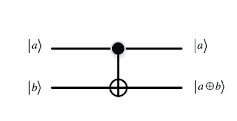
\includegraphics[width=\textwidth]{Figures/Xor.png}
    \caption{XOR using CNOT}
    \label{fig:xor_cnot}
\end{subfigure}
\hfill
\begin{subfigure}[t]{0.47\textwidth}
    \centering
    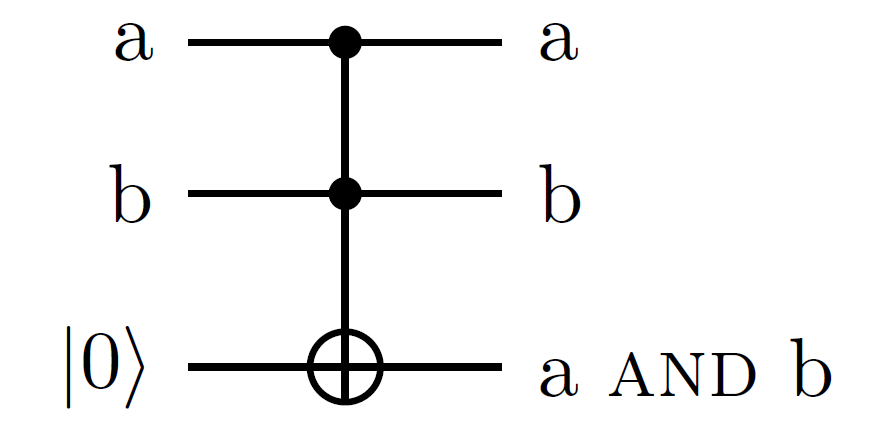
\includegraphics[width=\textwidth]{Figures/AND.png}
    \caption{AND using CCNOT/Toffoli}
    \label{fig:and_toffoli}
\end{subfigure}
\caption{Reversible implementation of XOR and AND operations using elementary quantum gates \cite{nielsen2010quantum,barenco1995elementary,toffoli1980reversible}}
\label{fig:xor_and_gates}
\end{figure}

\subsection{Classical PRINCE Cipher}

PRINCE is a lightweight symmetric block cipher designed for latency-sensitive cryptographic applications. It operates on a 64-bit plaintext block and uses a 128-bit secret key. Unlike several lightweight ciphers that primarily optimize area or energy consumption, PRINCE was designed to minimize encryption latency in hardware, especially for fully unrolled implementations \cite{borghoff2012prince}. Subsequent work has analyzed its security properties and related-key behavior \cite{jean2013security}. The high-level circuit organization of PRINCE is shown in Figure~\ref{fig:prince_circuit_design}.

\begin{figure}[H]
\centering
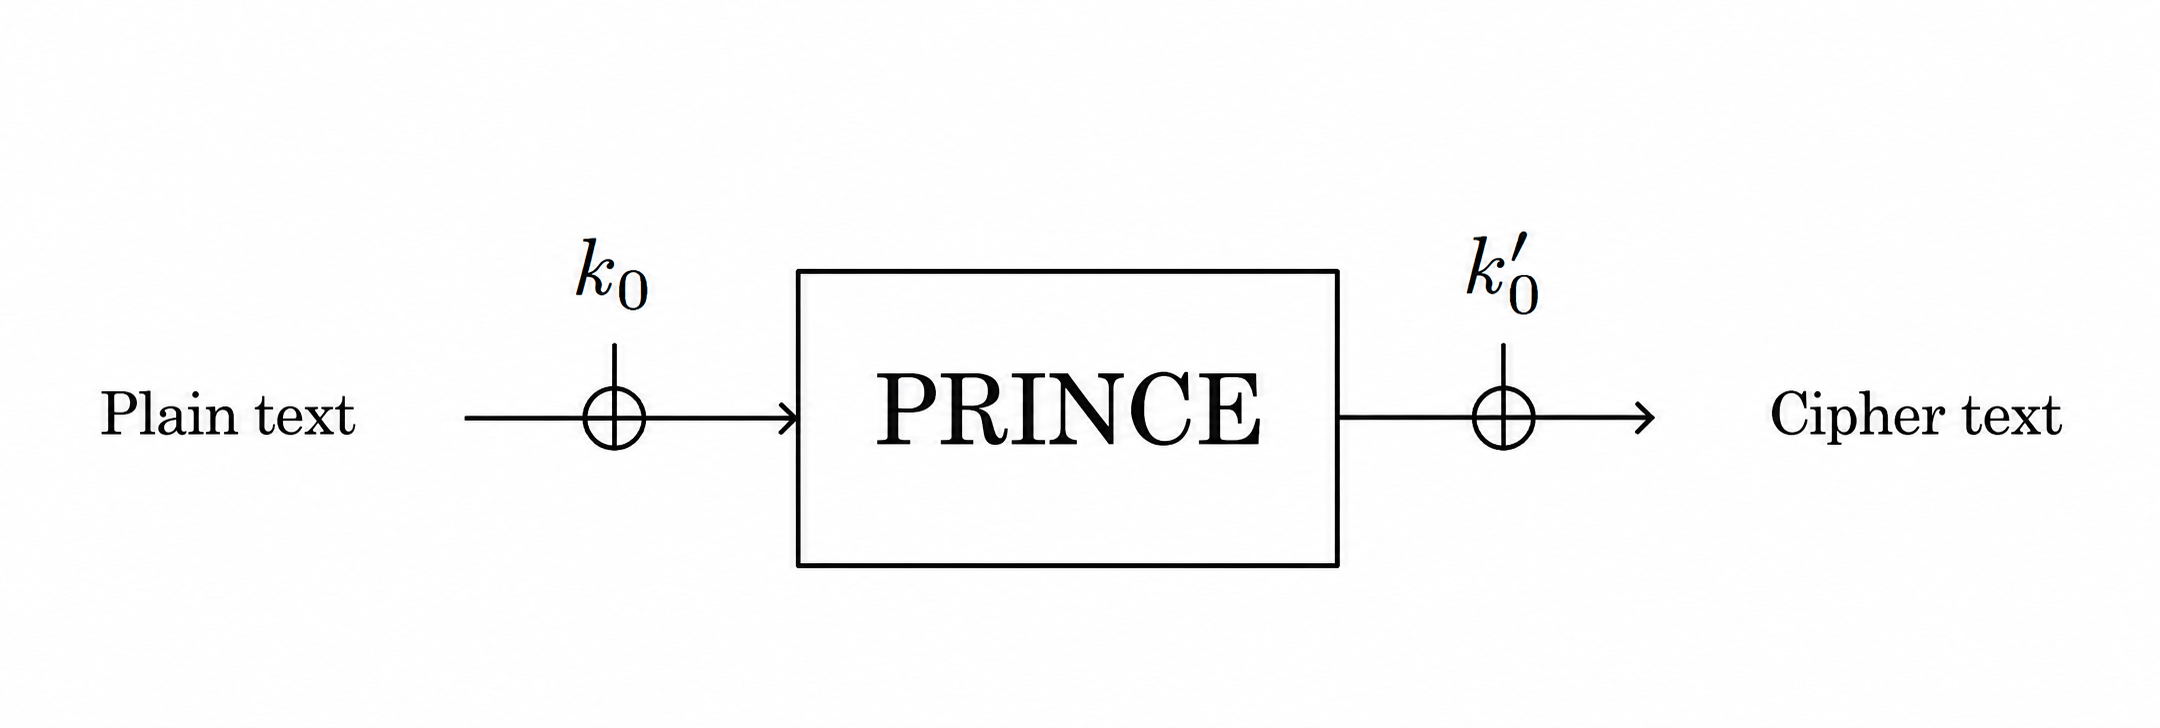
\includegraphics[width=0.7\textwidth]{Figures/Prince_Circuit_Design.png}
\caption{Circuit design structure of the PRINCE block cipher \cite{borghoff2012prince}}
\label{fig:prince_circuit_design}
\end{figure}

The general structure of PRINCE consists of initial whitening, five forward rounds, a middle layer, five inverse rounds, and final whitening \cite{borghoff2012prince}. The 128-bit master key is divided into two 64-bit subkeys, denoted by $k_0$ and $k_1$. The value $k_0$ is used during the initial whitening step, while a derived key $k_0'$ is used during the final whitening step. The round key $k_1$ is used throughout the forward and inverse rounds. Each forward round applies four main operations: S-layer substitution, M-layer diffusion, round constant addition, and round-key addition. After the five forward rounds and the middle transformation, the inverse rounds are applied in reverse structural order. The overall PRINCE encryption structure is shown in Figure~\ref{fig:classical_prince_full}.

\begin{figure}[H]
\centering
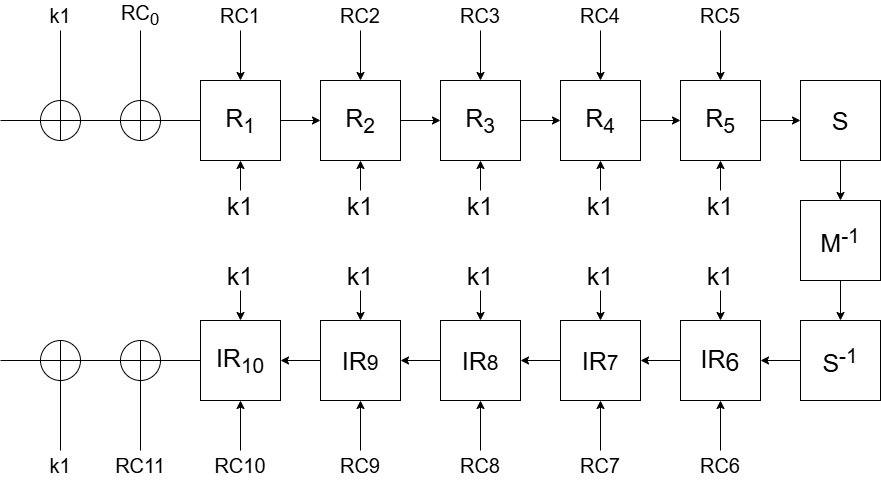
\includegraphics[width=0.85\textwidth]{Figures/Prince_Full.png}
\caption{Overall structure of the PRINCE block cipher \cite{borghoff2012prince}}
\label{fig:classical_prince_full}
\end{figure}

The S-layer is the nonlinear substitution layer of PRINCE and provides confusion in the cipher. In this layer, the 64-bit internal state is divided into sixteen independent 4-bit nibbles, and each nibble is transformed using the PRINCE S-box \cite{borghoff2012prince}. The S-box maps each 4-bit input to a 4-bit output, making the relation between plaintext, key, and ciphertext nonlinear. The S-box mapping used in PRINCE is given in Table~\ref{tab:classical_prince_sbox}.

\begin{table}[H]
\centering
\caption{PRINCE S-box mapping \cite{borghoff2012prince}}
\label{tab:classical_prince_sbox}
\begin{tabular}{|c|c|c|c|}
\hline
\textbf{Input (Hex)} & \textbf{Input (Bin)} & \textbf{Output (Hex)} & \textbf{Output (Bin)} \\
\hline
0x0 & 0000 & 0xB & 1011 \\
\hline
0x1 & 0001 & 0xF & 1111 \\
\hline
0x2 & 0010 & 0x3 & 0011 \\
\hline
0x3 & 0011 & 0x2 & 0010 \\
\hline
0x4 & 0100 & 0xA & 1010 \\
\hline
0x5 & 0101 & 0xC & 1100 \\
\hline
0x6 & 0110 & 0x9 & 1001 \\
\hline
0x7 & 0111 & 0x1 & 0001 \\
\hline
0x8 & 1000 & 0x6 & 0110 \\
\hline
0x9 & 1001 & 0x7 & 0111 \\
\hline
0xA & 1010 & 0x8 & 1000 \\
\hline
0xB & 1011 & 0x0 & 0000 \\
\hline
0xC & 1100 & 0xE & 1110 \\
\hline
0xD & 1101 & 0x5 & 0101 \\
\hline
0xE & 1110 & 0xD & 1101 \\
\hline
0xF & 1111 & 0x4 & 0100 \\
\hline
\end{tabular}
\end{table}

The M-layer is the linear diffusion layer of PRINCE. Its purpose is to spread the effect of individual state bits across the internal state so that a small change in the plaintext or key affects many output bits after multiple rounds \cite{borghoff2012prince}. The transformation is defined over $GF(2)$ and can be represented using binary matrices. The 64-bit state is divided into four 16-bit blocks, and each block is transformed using the matrix $M_{16}$. The complete M-layer matrix is then formed as a block diagonal matrix according to the PRINCE specification \cite{borghoff2012prince}.

\[
I_4 =
\begin{bmatrix}
1 & 0 & 0 & 0 \\
0 & 1 & 0 & 0 \\
0 & 0 & 1 & 0 \\
0 & 0 & 0 & 1
\end{bmatrix}
\qquad
Z_4 =
\begin{bmatrix}
0 & 0 & 0 & 0 \\
0 & 0 & 0 & 0 \\
0 & 0 & 0 & 0 \\
0 & 0 & 0 & 0
\end{bmatrix}
M_{16} =
\begin{bmatrix}
Z_4 & I_4 & I_4 & I_4 \\
I_4 & Z_4 & I_4 & I_4 \\
I_4 & I_4 & Z_4 & I_4 \\
I_4 & I_4 & I_4 & Z_4
\end{bmatrix}
\]

\vspace{0.6cm}
\[
M =
\begin{bmatrix}
M_{16} & 0 & 0 & 0 \\
0 & M_{16} & 0 & 0 \\
0 & 0 & M_{16} & 0 \\
0 & 0 & 0 & M_{16}
\end{bmatrix}_{64 \times 64}
\]

Since the M-layer is linear, it consists only of XOR-based transformations and does not introduce nonlinear terms. Thus, in the quantum implementation, it can be realized using CNOT gates, while the nonlinear S-layer requires Toffoli gates for product terms. Together, the S-layer and M-layer form the substitution--permutation core of PRINCE, and the surrounding whitening and key schedule operations complete the classical cipher structure \cite{borghoff2012prince}.

\subsection{Grover's Algorithm}

Grover's algorithm is a quantum search algorithm for finding a marked element in an unstructured search space. Classically, if the search space contains $N$ possible candidates and only one candidate is correct, exhaustive search requires $O(N)$ evaluations in the worst case. Grover's algorithm reduces this to $O(\sqrt{N})$ oracle queries by repeatedly amplifying the amplitude of the marked state \cite{grover1996fast,grover1997quantum,boyer1998tight,brassard2002amplitude}. This quadratic speedup is the main reason why Grover's algorithm is important in the analysis of symmetric-key cryptography.

The algorithm begins by preparing a uniform superposition over all possible inputs. For a search space of size $N=2^n$, the initial state is
\[
|s\rangle =
\frac{1}{\sqrt{N}}
\sum_{x=0}^{N-1} |x\rangle .
\]
An oracle $O_f$ is then used to identify the correct solution. If $f(x)=1$ for the marked item and $f(x)=0$ otherwise, the phase oracle acts as
\[
O_f |x\rangle = (-1)^{f(x)} |x\rangle .
\]
Thus, the oracle does not directly reveal the solution; instead, it flips the phase of the marked state while leaving all unmarked states unchanged \cite{nielsen2010quantum}.

After the oracle, Grover's algorithm applies the diffusion operator, also called inversion about the mean \cite{grover1997quantum,nielsen2010quantum}. The diffuser is written as
\[
D = 2|s\rangle\langle s| - I .
\]
One Grover iteration consists of applying the oracle followed by the diffuser:
\[
G = D O_f .
\]
Geometrically, this repeated operation rotates the quantum state toward the marked solution subspace. When there is one marked item, the number of iterations required to obtain the marked state with high probability is approximately
\[
r \approx \left\lfloor \frac{\pi}{4}\sqrt{N} \right\rfloor .
\]
More generally, if there are $M$ marked items in a search space of size $N$, the query complexity becomes $O(\sqrt{N/M})$ \cite{boyer1998tight}.

In symmetric-key cryptanalysis, the search space is the key space. For a block cipher with a $k$-bit key, there are $N=2^k$ possible keys. Given a known plaintext--ciphertext pair $(P,C)$, the Grover oracle marks a candidate key $K$ if the encryption relation $E_K(P)=C$ holds. Therefore, a quantum exhaustive key-search attack requires approximately $O(2^{k/2})$ Grover iterations rather than $O(2^k)$ classical trials \cite{grassl2016applying,kim2018timespace}. For PRINCE, where $k=128$, this means that the ideal key-search security is reduced from 128 bits to about 64 bits. However, every Grover iteration must include a reversible implementation of the cipher, ciphertext comparison, phase marking, uncomputation, and diffusion. Hence, the practical feasibility of the attack depends not only on the asymptotic iteration count, but also on the gate count, qubit count, circuit depth, T-count, and T-depth of the implemented oracle.

\section{Reversible PRINCE Cipher}

This section describes the construction of a reversible quantum circuit for the PRINCE block cipher. Since quantum operations must be unitary and reversible, the classical PRINCE encryption structure cannot be used directly as an irreversible Boolean computation \cite{nielsen2010quantum}. Instead, each component of PRINCE, including key whitening, round-key addition, round constants, the S-layer, the M-layer, and the key schedule, is translated into reversible operations based mainly on X, CNOT, and Toffoli gates. The goal of this construction is to preserve the classical behavior of PRINCE \cite{borghoff2012prince} while producing a clean reversible oracle that can later be embedded into Grover's key-search algorithm.

\subsection{Qubit Distribution}

The quantum implementation of PRINCE uses separate qubit registers for storing the plaintext state, secret key components, and ancilla workspace required for reversible operations. This register separation follows the standard reversible-computation requirement that intermediate information must be preserved or explicitly uncomputed instead of being erased \cite{bennett1973logical,nielsen2010quantum}. The 64-bit state register stores the plaintext and all intermediate values generated during encryption. Additional ancilla qubits are required mainly for reversible S-box computation, where temporary values must be stored without destroying the original input state. Separate registers are also maintained for the PRINCE key components $k_0$, $k_1$, and the derived key $k_0'$ defined by the classical cipher specification \cite{borghoff2012prince}.

\begin{table}[H]
\centering
\caption{Qubit allocation in the proposed quantum PRINCE implementation}
\label{tab:qubit_distribution}
\begin{tabular}{|c|c|p{7cm}|}
\hline
\textbf{Qubit Range} & \textbf{Purpose} & \textbf{Description} \\
\hline
0--63 & State Register & Stores the 64-bit plaintext and intermediate cipher state during encryption \\
\hline
64--287 & S-box Ancilla & Ancilla workspace used during reversible implementation of the S-box layer \\
\hline
288--351 & $k_0$ Register & Stores the first 64-bit key half used during initial whitening \\
\hline
352--415 & $k_1$ Register & Stores the round key used in all forward and inverse rounds \\
\hline
416--479 & $k_0'$ Register & Stores the derived key used during final whitening \\
\hline
\end{tabular}
\end{table}

The separation of registers helps preserve reversibility throughout the computation. The ancilla qubits used during intermediate computations are uncomputed back to the $|0\rangle$ state after use, ensuring that no unwanted garbage states remain in the circuit \cite{bennett1973logical}. This property is essential for embedding the encryption circuit into Grover's algorithm, where the oracle must be reversible and must not leave residual information entangled with the key register \cite{nielsen2010quantum,grassl2016applying}.

\subsection{Quantum Round Constants and Key Addition}

Round constants and key addition in PRINCE are XOR-based operations. In the classical cipher, a 64-bit round constant $RC_i$ is XORed into the 64-bit internal state during each round, and the appropriate key material is also XORed into the state during whitening and round-key addition \cite{borghoff2012prince}. Since XOR is reversible, these operations are direct to implement in a quantum circuit. For a known constant bit equal to 1, round-constant addition is implemented by applying a Pauli-X gate to the corresponding state qubit; if the constant bit is 0, no gate is applied. For key addition, each key bit is XORed into the corresponding state bit using a CNOT gate, where the key qubit is the control and the state qubit is the target \cite{nielsen2010quantum,barenco1995elementary}.

\begin{table}[H]
\centering
\caption{PRINCE round constants \cite{borghoff2012prince}}
\label{tab:prince_round_constants}
\begin{tabularx}{\textwidth}{|>{\centering\arraybackslash}X|>{\centering\arraybackslash}X|}
\hline
\textbf{Round Constant} & \textbf{64-bit Hexadecimal Value} \\
\hline
$RC_0$ & 0x0000000000000000 \\
\hline
$RC_1$ & 0x13198A2E03707344 \\
\hline
$RC_2$ & 0xA4093822299F31D0 \\
\hline
$RC_3$ & 0x082EFA98EC4E6C89 \\
\hline
$RC_4$ & 0x452821E638D01377 \\
\hline
$RC_5$ & 0xBE5466CF34E90C6C \\
\hline
$RC_6$ & 0x7EF84F78FD955CB1 \\
\hline
$RC_7$ & 0x85840851F1AC43AA \\
\hline
$RC_8$ & 0xC882D32F25323C54 \\
\hline
$RC_9$ & 0x64A51195E0E3610D \\
\hline
$RC_{10}$ & 0xD3B5A399CA0C2399 \\
\hline
$RC_{11}$ & 0xC0AC29B7C97C50DD \\
\hline
\end{tabularx}
\end{table}

Thus, round-constant addition does not require CNOT or Toffoli gates because the constants are public fixed values; it only requires X gates on the state positions where the selected constant has a 1-bit. Key addition, on the other hand, depends on the unknown key register, so it is implemented using CNOT gates. For a state bit $s_i$ and key bit $k_i$, the operation is
\[
s_i \leftarrow s_i \oplus k_i,
\]
which corresponds to $\mathrm{CNOT}(k_i,s_i)$ in the reversible circuit. Applying the same CNOT sequence again uncomputes the key addition, which is required when the PRINCE oracle is reversed during Grover iteration.

\begin{figure}[h]
    \centering
    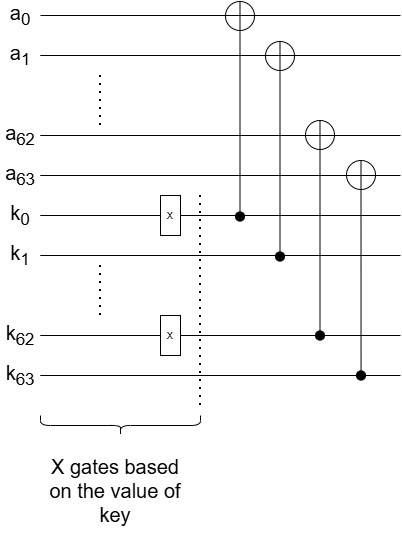
\includegraphics[width=0.5\linewidth]{Figures/key_round_constants.png}
    \caption{Quantum circuit for adding keys and round constants }
    \label{fig:keys_rounds_addition}
\end{figure}

\subsection{Quantum Round Structure}

The reversible PRINCE circuit follows the same high-level structure as the classical cipher. The encryption process begins with initial key whitening, followed by five forward rounds, a middle layer, and five inverse rounds. Finally, a last whitening stage is applied using the derived key material, preserving the round organization and reflection-based structure of PRINCE \cite{borghoff2012prince}.

The inverse rounds apply the inverse transformations in reverse order while preserving reversibility. Since XOR operations are naturally reversible, round-key addition and round constant addition are implemented efficiently using CNOT and Pauli-X gates \cite{nielsen2010quantum,barenco1995elementary}. This makes the linear and key-addition parts of the cipher comparatively direct to translate into a quantum circuit.

\begin{figure}[H]
\centering
\begin{subfigure}[t]{0.47\textwidth}
    \centering
    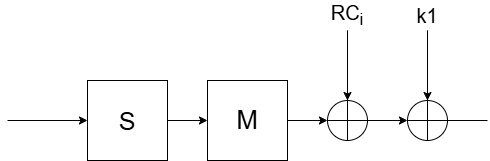
\includegraphics[width=\textwidth]{Figures/Forward_Round.png}
    \caption{Quantum Forward Round Structure of PRINCE}
    \label{fig:Forward_prince}
\end{subfigure}
\hfill
\begin{subfigure}[t]{0.47\textwidth}
    \centering
    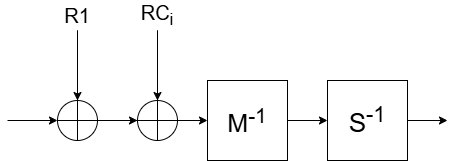
\includegraphics[width=\textwidth]{Figures/Backward_Round.png}
    \caption{Quantum Inverse Round Structure of PRINCE}
    \label{fig:Backward_prince}
\end{subfigure}
\caption{Forward and inverse round structures used in the reversible PRINCE circuit \cite{borghoff2012prince}}
\label{fig:Prince_Rounds}
\end{figure}

The middle layer connects the forward and inverse halves of the cipher and consists of an S-layer, M-layer, and inverse S-layer. Together, these components preserve the reflection-based structure of PRINCE while remaining compatible with reversible quantum computation \cite{borghoff2012prince,bennett1973logical}.

\subsection{Quantum Key Generation}

The PRINCE key schedule is implemented reversibly using quantum operations. According to the PRINCE specification, the 128-bit master key is divided into two 64-bit halves, denoted as $k_0$ and $k_1$, and a modified whitening key $k_0'$ is generated from $k_0$ using a one-bit circular right rotation followed by XOR with the most significant bit \cite{borghoff2012prince}.

\begin{figure}[H]
\centering
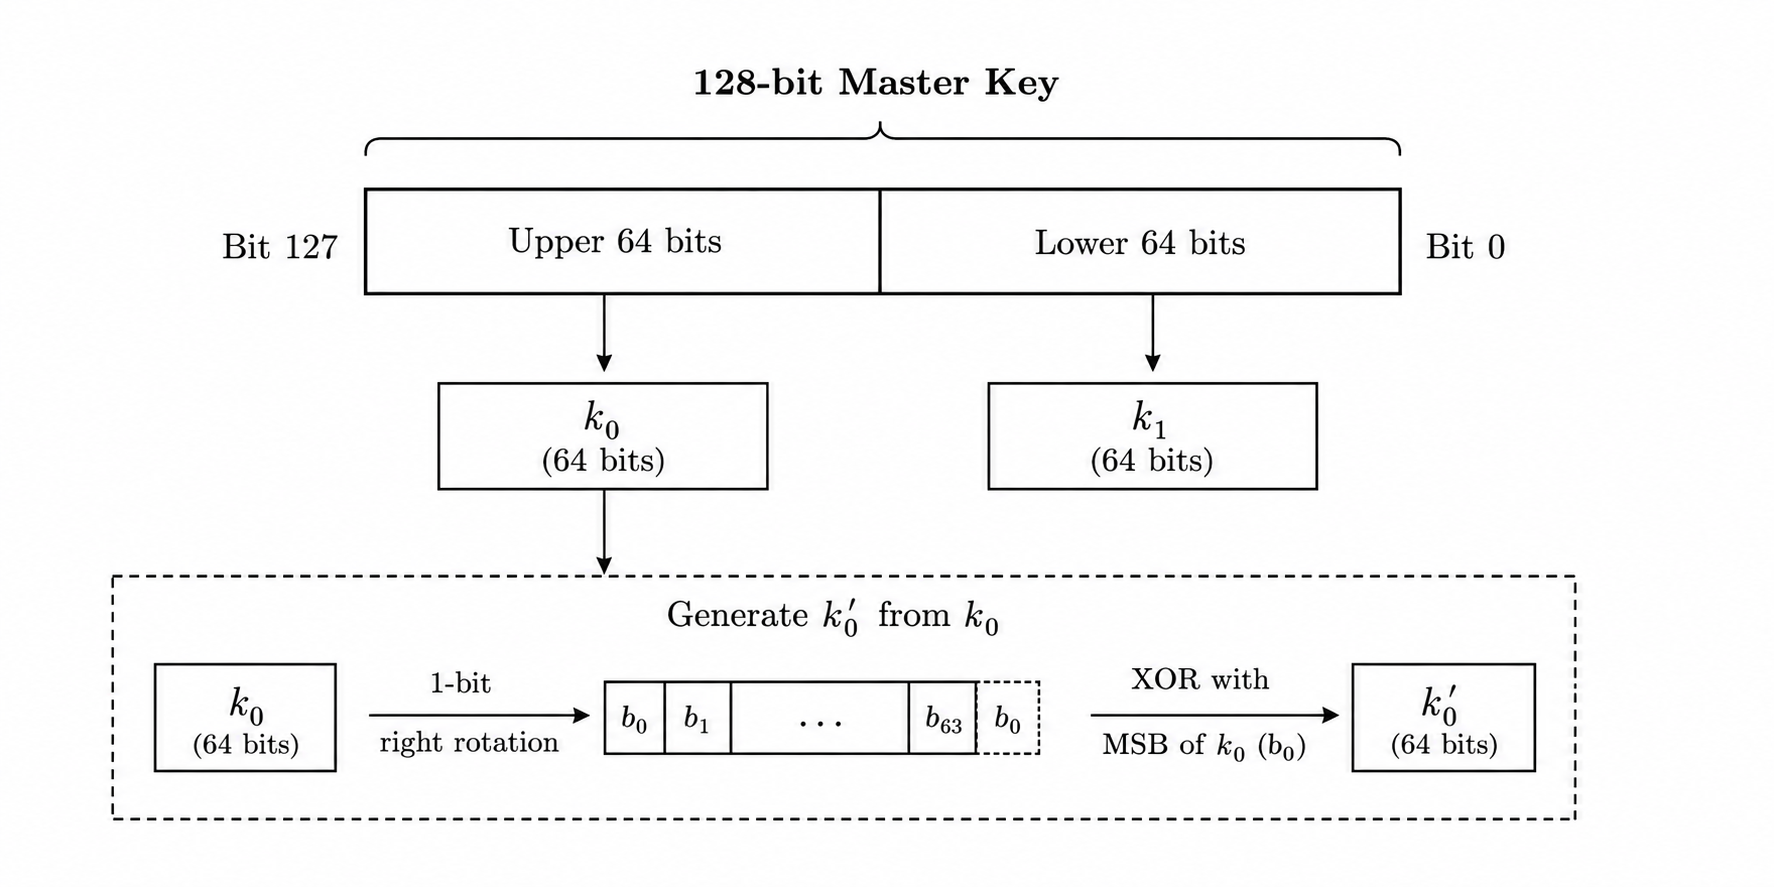
\includegraphics[width=\textwidth]{Figures/Key_Generation.png}
\caption{Quantum key generation structure for PRINCE \cite{borghoff2012prince}}
\label{fig:quantum_key_generation}
\end{figure}

The generated key material is stored in dedicated quantum registers and reused during the whitening and round-key addition stages. Since the operations used in this part of the key schedule are XOR-based, they can be implemented reversibly using CNOT gates without requiring large additional ancilla resources \cite{nielsen2010quantum,barenco1995elementary}. This keeps the key-generation part compatible with later oracle uncomputation in Grover search \cite{grassl2016applying}.

\subsection{Quantum S-box Implementation}

The S-box is the only non-linear component of the PRINCE cipher and therefore represents one of the most important parts of the reversible quantum implementation. In the PRINCE S-layer, the 64-bit state is divided into sixteen 4-bit nibbles, and the same 4-bit substitution is applied independently to each nibble \cite{borghoff2012prince}.

Direct lookup-table implementation is not suitable in quantum computation because quantum operations must be reversible and cannot overwrite unknown quantum states \cite{nielsen2010quantum,bennett1973logical}. Therefore, the PRINCE S-box is represented using Algebraic Normal Form (ANF), where each output bit is expressed as a Boolean polynomial over $GF(2)$ using XOR terms and product terms over the input bits. ANF is a standard representation for Boolean functions in cryptography, and the ANF coefficients can be obtained from the truth table using the Mobius transform \cite{rota1964mobius,carlet2021boolean}. The representative ANF coefficient calculation and the final ANF equations used for the PRINCE S-box are shown in Figure~\ref{fig:anf_combined}.

\begin{figure}[H]
\centering
\fbox{
\begin{minipage}{0.92\textwidth}
\setlength{\abovedisplayskip}{3pt}
\setlength{\belowdisplayskip}{3pt}
\begin{align*}
f(a_3,a_2,a_1,a_0)
&= C_0 \oplus C_1a_0 \oplus C_2a_1 \oplus C_3a_0a_1
 \oplus C_4a_2 \oplus C_5a_0a_2 \oplus C_6a_1a_2 \oplus C_7a_0a_1a_2 \\
&\quad \oplus C_8a_3 \oplus C_9a_0a_3 \oplus C_{10}a_1a_3
 \oplus C_{11}a_0a_1a_3 \oplus C_{12}a_2a_3 \\
&\quad \oplus C_{13}a_0a_2a_3 \oplus C_{14}a_1a_2a_3
 \oplus C_{15}a_0a_1a_2a_3 \\[6pt]
& \text{(Mobius transformation is used to obtain these constants)} \\[8pt]
C_0 &= f(0000) = 1 \\
C_1 &= f(0001) \oplus f(0000) = 1 \oplus 1 = 0 \\
C_3 &= f(0011) \oplus f(0010) \oplus f(0001) \oplus f(0000)
     = 0 \oplus 1 \oplus 1 \oplus 1 = 1 \\
C_4 &= f(0100) \oplus f(0000) = 0 \oplus 1 = 1 \\
C_6 &= f(0110) \oplus C_0 \oplus C_2 \oplus C_4
     = 1 \oplus 1 \oplus 0 \oplus 1 = 1 \\
C_8 &= f(1000) \oplus f(0000) = 0 \oplus 1 = 1 \\
&\quad \vdots \quad \text{(remaining } C_i \text{ computed similarly; } C_{10}=C_{11}=\cdots=C_{15}=0 \text{)} \\[8pt]
b_0 &= 1
  \oplus a_0a_1
  \oplus a_2
  \oplus a_1a_2
  \oplus a_0a_1a_2
  \oplus a_3
  \oplus a_0a_3 \\[4pt]
b_1 &= 1
  \oplus a_0a_2
  \oplus a_1a_2
  \oplus a_0a_1a_2
  \oplus a_0a_3
  \oplus a_1a_3
  \oplus a_2a_3 \\[4pt]
b_2 &= a_0
  \oplus a_0a_1
  \oplus a_3
  \oplus a_0a_3
  \oplus a_1a_3
  \oplus a_0a_2a_3
  \oplus a_1a_2a_3 \\[4pt]
b_3 &= 1
  \oplus a_1
  \oplus a_1a_2
  \oplus a_0a_1a_2
  \oplus a_3
  \oplus a_1a_3
  \oplus a_0a_1a_3
  \oplus a_2a_3
\end{align*}
\end{minipage}
}
\caption{ANF coefficient calculation using the Mobius transform and final ANF equations for the PRINCE S-box output bits \cite{borghoff2012prince,rota1964mobius,carlet2021boolean}}
\label{fig:anf_combined}
\end{figure}


The ANF representation is suitable for quantum implementation because XOR operations can be implemented using CNOT gates, constant bit flips can be implemented using Pauli-X gates, and product terms can be implemented using Toffoli gates \cite{toffoli1980reversible,barenco1995elementary}. This mapping converts the nonlinear PRINCE S-box into a reversible quantum circuit while preserving the original S-box behavior.

The resulting reversible S-box circuit is implemented using a combination of Pauli-X, CNOT, and Toffoli gates. Temporary ancilla qubits are used during intermediate computations and are later uncomputed to maintain reversibility \cite{bennett1973logical,nielsen2010quantum}.

\begin{table}[H]
\centering
\caption{Quantum Resource Requirement for One PRINCE S-layer}
\label{tab:sbox_resource}
\begin{tabular}{|c|c|p{7cm}|}
\hline
\textbf{Resource} & \textbf{Count} & \textbf{Description} \\
\hline
S-box Instances & 16 & One S-box is applied independently to each 4-bit nibble of the 64-bit state \\
\hline
Input Qubits & 64 & State qubits used as input to the S-layer \\
\hline
Ancilla Qubits & 224 & Temporary workspace qubits required for reversible ANF computation \\
\hline
Pauli-X Gates & 80 & Used for constant bit flips in the ANF implementation \\
\hline
CNOT Gates & 880 & Used for XOR operations in the reversible S-box computation \\
\hline
Toffoli Gates & 640 & Used for implementing non-linear product terms in the ANF equations \\
\hline
Total Quantum Gates & 1600 & Total number of gates required for one complete S-layer \\
\hline
\end{tabular}
\end{table}

\begin{figure}[H]
\centering
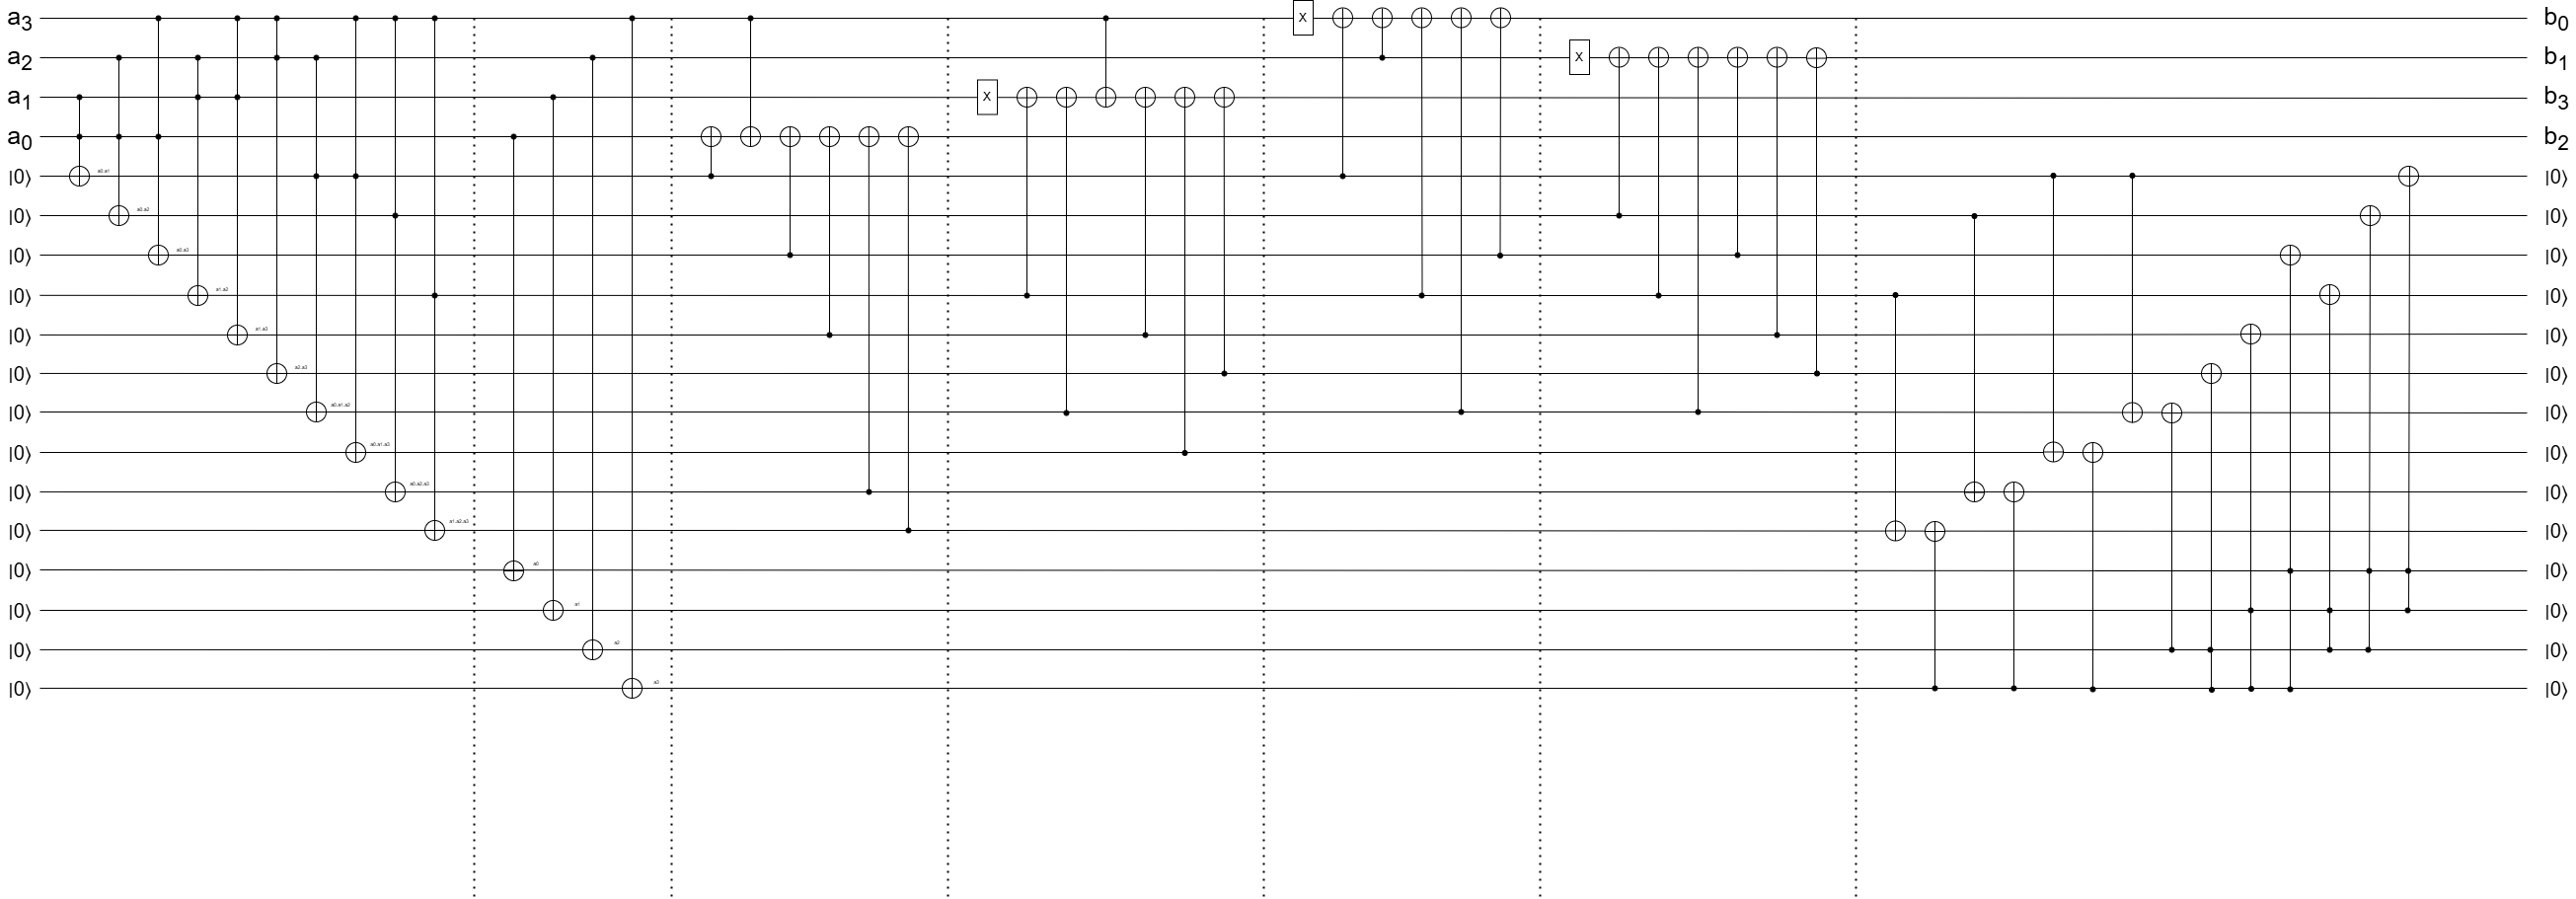
\includegraphics[width=\linewidth]{Figures/S-nibble.png}
\caption{Reversible quantum circuit for the PRINCE S-box constructed from the ANF equations}
\label{fig:quantum_sbox_circuit}
\end{figure}

The PRINCE S-layer operates on the complete 64-bit internal state by dividing it into sixteen independent 4-bit nibbles. Each nibble is processed using the reversible ANF-based S-box circuit shown in Figure~\ref{fig:quantum_sbox_circuit}. Since the same S-box structure is reused for all sixteen nibbles, the total resource requirement of one S-layer is obtained by multiplying the resource cost of a single S-box by sixteen. The S-layer contributes significantly to the overall quantum resource cost of the PRINCE circuit because the nonlinear ANF terms require Toffoli gates and ancilla qubits \cite{akhlaq2024quantum,barenco1995elementary}.

\subsection{Quantum M-box Implementation}

The M-box is the linear diffusion layer of PRINCE and is responsible for spreading bit changes across the internal state \cite{borghoff2012prince}. Unlike the S-box, the M-box contains only linear XOR-based operations, so it can be implemented using only CNOT gates. This follows the standard synthesis view of linear reversible circuits: an invertible binary matrix over $GF(2)$ can be realized as a sequence of CNOT gates, and Gaussian elimination gives a direct way to obtain such a sequence \cite{patel2008optimal}. Figure~\ref{fig:gaussian_mbox} shows why Gaussian elimination is useful for in-place M-box implementation.

\begin{figure}[h]
\centering
\fbox{
\begin{minipage}{0.88\textwidth}
\setlength{\abovedisplayskip}{3pt}
\setlength{\belowdisplayskip}{3pt}
\begin{align*}
y &= Mx, \qquad M \in GF(2)^{64 \times 64} \\[2pt]
R_i &\leftarrow R_i \oplus R_j
\end{align*}

Over $GF(2)$, adding row $R_j$ to row $R_i$ is the same as XORing the
corresponding values. In a quantum circuit, this row operation is implemented as:

\[
\text{CNOT}(q_j, q_i): \quad q_i \leftarrow q_i \oplus q_j
\]

Gaussian elimination reduces the matrix $M$ to the identity matrix:

\[
E_t E_{t-1} \cdots E_2 E_1 M = I
\]

where each $E_i$ is an elementary row-operation matrix. Therefore,

\[
M = E_1^{-1} E_2^{-1} \cdots E_{t-1}^{-1} E_t^{-1}
\]

Since XOR row operations are self-inverse over $GF(2)$,

\[
E_i^{-1} = E_i
\]

Hence,

\[
M = E_1 E_2 \cdots E_t
\]
\end{minipage}
}
\caption{Gaussian elimination method for in-place M-box implementation \cite{patel2008optimal}}
\label{fig:gaussian_mbox}
\end{figure}

Since row XOR operations over $GF(2)$ are self-inverse, the same elementary operations can be applied in reverse order to synthesize the original matrix transformation $M$ \cite{patel2008optimal}.

Each Gaussian-elimination row operation maps directly to a CNOT gate. A row operation
\[
R_i \leftarrow R_i \oplus R_j
\]
corresponds to the quantum gate
\[
\mathrm{CNOT}(q_j,q_i):\qquad q_i \leftarrow q_i \oplus q_j,
\]

where $q_j$ is the control qubit and $q_i$ is the target qubit. Thus, every XOR row update in the elimination sequence contributes one CNOT gate to the M-box circuit. The method is in-place: it updates the 64 state qubits directly and does not require a separate output register or ancilla qubits. The relationship between Gaussian elimination and CNOT synthesis is summarized in Figure~\ref{fig:gaussian_mbox}.

The final M-box circuit therefore realizes the PRINCE diffusion matrix as a reversible in-place linear transformation. Because the transformation is linear over $GF(2)$, it uses only CNOT gates; because Gaussian elimination reduces the input matrix to the identity and records each row-XOR operation, the recorded operations directly determine the CNOT sequence for the circuit. This satisfies the reversibility requirement of the Grover oracle while keeping the M-layer free of ancilla and Toffoli gates \cite{bennett1973logical,nielsen2010quantum}.

As shown in Figure~\ref{fig:gaussian_mbox}, Gaussian elimination generates a sequence of elementary matrices
\[
E_1,E_2,\ldots,E_n
\]
whose product represents the M-box transformation. Each elementary row-addition matrix corresponds to one CNOT operation, while row exchanges can be implemented using swap operations or decomposed into elementary reversible gates \cite{nielsen2010quantum,patel2008optimal}. Figure~\ref{fig:matrix_to_circuit} illustrates the conversion of an elementary matrix operation into a circuit operation, and Figure~\ref{fig:swap} shows a swap operation used when row exchange is required. Applying the resulting sequence of CNOT gates implements the PRINCE M-box, whose complete circuit is shown in Figure~\ref{fig:quantum_mbox}.

\begin{figure}[H]
\centering
\begin{subfigure}[t]{0.47\textwidth}
    \centering
    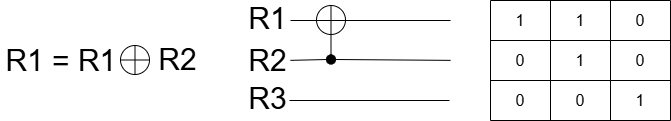
\includegraphics[width=\textwidth]{Figures/matrix_to_circuit.png}
    \caption{Elementary matrix operation converted to a CNOT-based circuit}
    \label{fig:matrix_to_circuit}
\end{subfigure}
\hfill
\begin{subfigure}[t]{0.47\textwidth}
    \centering
    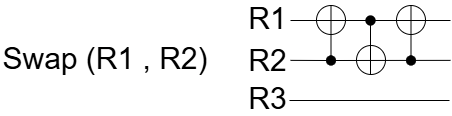
\includegraphics[width=\textwidth]{Figures/Swap.png}
    \caption{Swap operation used for exchanging two lines}
    \label{fig:swap}
\end{subfigure}
\caption{Useful reversible operations for converting elementary matrix operations into a quantum circuit using a conceptually miniature 3-bit example \cite{nielsen2010quantum,patel2008optimal}}
\label{fig:matrix_ops_to_circuit}
\end{figure}

\begin{table}[h]
\centering
\caption{Quantum resource requirement for one PRINCE M-layer}
\label{tab:mbox_resource}
\begin{tabular}{|c|c|p{7cm}|}
\hline
\textbf{Resource} & \textbf{Count} & \textbf{Description} \\
\hline
Input Qubits & 64 & State qubits representing the 64-bit PRINCE internal state \\
\hline
Ancilla Qubits & 0 & The M-layer is implemented in-place without requiring additional ancilla qubits \\
\hline
Pauli-X Gates & 0 & No constant bit inversions are required in the linear diffusion layer \\
\hline
CNOT Gates & 224 & Used to realize the linear matrix transformation through Gaussian elimination \\
\hline
Toffoli Gates & 0 & The M-layer contains only linear XOR operations and therefore requires no nonlinear gates \\
\hline
Total Quantum Gates & 224 & Total number of quantum gates required for one complete M-layer \\
\hline
\end{tabular}
\end{table}

\begin{figure}[H]
\centering

\includegraphics[width=\linewidth]{Figures/Mbox.png}
\caption{Quantum circuit implementation of the PRINCE M-box synthesized from Gaussian-elimination row operations \cite{borghoff2012prince,patel2008optimal}}
\label{fig:quantum_mbox}
\end{figure}

\subsection{Round-wise Gate Distribution}

The gate count of the PRINCE circuit is analyzed round by round. Each forward and inverse round contains an S-layer, M-layer, round constant addition, and key addition. The number of CNOT and Toffoli gates remains fixed for each round, while the number of X gates changes depending on the Hamming weight of the round constant.

\begin{table}[h]
\centering
\caption{Round-wise Gate Distribution of PRINCE}
\label{tab:round_gate_distribution}
\begin{tabular}{|c|c|c|c|c|}
\hline
\textbf{Stage} & \textbf{X Gates} & \textbf{CNOT Gates} & \textbf{Toffoli Gates} & \textbf{Total Gates} \\
\hline
Initial Key Addition & 0 & 128 & 0 & 128 \\
\hline
Round 1 & 105 & 1168 & 640 & 1913 \\
\hline
Round 2 & 105 & 1168 & 640 & 1913 \\
\hline
Round 3 & 110 & 1168 & 640 & 1918 \\
\hline
Round 4 & 107 & 1168 & 640 & 1915 \\
\hline
Round 5 & 113 & 1168 & 640 & 1921 \\
\hline
Middle Layer & 160 & 1984 & 1280 & 3424 \\
\hline
Inverse Round 6 & 119 & 1168 & 640 & 1927 \\
\hline
Inverse Round 7 & 105 & 1168 & 640 & 1913 \\
\hline
Inverse Round 8 & 108 & 1168 & 640 & 1916 \\
\hline
Inverse Round 9 & 107 & 1168 & 640 & 1915 \\
\hline
Inverse Round 10 & 111 & 1168 & 640 & 1919 \\
\hline
Final Whitening & 32 & 128 & 0 & 160 \\
\hline
\textbf{Total} & \textbf{1282} & \textbf{13920} & \textbf{7680} & \textbf{22882} \\
\hline
\end{tabular}
\end{table}

\section{Results and Discussion}

This section reports the resource estimates obtained for the reversible PRINCE implementation and its use inside Grover key search. The tables are organized in the following order: resources for the PRINCE cipher, resources for one Grover iteration, and resources for all Grover iterations. The same order is then repeated for the Clifford+T resource group. Full-state simulation over the complete PRINCE key space is infeasible because the key register ranges over $2^{128}$ candidates, so the full-attack estimates are obtained by multiplying the one-iteration resource cost by the standard Grover iteration count \cite{grover1996fast,boyer1998tight,grassl2016applying}.


\subsection{Standard Gate Resources}

\begin{table}[H]
\centering
\caption{Resource requirements for the reversible PRINCE cipher}
\label{tab:result_prince_standard}
\begin{tabularx}{\textwidth}{|*{6}{>{\centering\arraybackslash}X|}}
\hline
\textbf{Qubits} & \textbf{X Gates} & \textbf{CNOT Gates} & \textbf{Toffoli Gates} & \textbf{Total Gates} & \textbf{Depth} \\
\hline
480 & 1282 & 13920 & 7680 & 22882 & 10712 \\
\hline
\end{tabularx}
\end{table}

\begin{table}[H]
\centering
\caption{Resource requirements for one PRINCE Grover iteration}
\label{tab:result_grover_one_standard}
\begin{tabularx}{\textwidth}{|*{8}{>{\centering\arraybackslash}X|}}
\hline
\textbf{Qubits} & \textbf{H} & \textbf{X} & \textbf{Z} & \textbf{CNOT} & \textbf{Toffoli} & \textbf{Total Gates} & \textbf{Depth} \\
\hline
607 & 384 & 2710 & 2 & 27970 & 15740 & 46806 & 2015 \\
\hline
\end{tabularx}
\end{table}

\subsection{Mathematical Gate Calculation}

The gate count for one Grover iteration is obtained by adding the resources required for plaintext loading, key superposition, oracle computation, ciphertext phase marking, oracle uncomputation, and the Grover diffuser. Since the PRINCE encryption circuit is used once for computation and once again for uncomputation, the PRINCE encryption resources appear twice in the Grover-iteration calculation. The component-wise mathematical gate calculation is shown in Table~\ref{tab:math_gate_calc_grover}.

\begin{table}[H]
\centering
\caption{Mathematical gate count calculation for one PRINCE Grover iteration}
\label{tab:math_gate_calc_grover}
\small
\renewcommand{\arraystretch}{1.25}
\begin{tabularx}{\textwidth}{|
>{\raggedright\arraybackslash}p{0.28\textwidth}|
>{\centering\arraybackslash}X|
>{\centering\arraybackslash}X|
>{\centering\arraybackslash}X|
>{\centering\arraybackslash}X|
>{\centering\arraybackslash}X|
>{\centering\arraybackslash}X|}
\hline
\textbf{Component} & \textbf{H} & \textbf{X} & \textbf{Z} & \textbf{CNOT} & \textbf{Toffoli} & \textbf{Total} \\
\hline
Plaintext loading & 0 & 16 & 0 & 0 & 0 & 16 \\
\hline
Key superposition & 128 & 0 & 0 & 0 & 0 & 128 \\
\hline
Compute and uncompute $k_0'$ & 0 & 0 & 0 & 130 & 0 & 130 \\
\hline
PRINCE encryption and uncomputation & 0 & 2564 & 0 & 27840 & 15360 & 45764 \\
\hline
Ciphertext phase marker & 0 & 198 & 1 & 0 & 126 & 325 \\
\hline
128-bit Grover diffuser & 256 & 256 & 1 & 0 & 254 & 511 \\
\hline
\textbf{Manual total} & \textbf{384} & \textbf{3034} & \textbf{2} & \textbf{27970} & \textbf{15740} & \textbf{47130} \\
\hline
\end{tabularx}
\end{table}

The manually calculated total gate count is 47,130, while the optimized Qiskit implementation reports 46,806 gates. Qiskit provides circuit construction, transpilation, and optimization functionality for quantum circuits \cite{qiskit2023}. In this case, the difference is caused by cancellation of some adjacent X gates during circuit optimization: the X-gate count decreases from 3,034 to 2,710, while the H, Z, CNOT, and Toffoli counts remain unchanged. Therefore, the optimized one-iteration value used in the final resource tables is 46,806 gates.

For the complete key search, the number of Grover iterations is estimated as
\[
I \approx \frac{\pi}{4}\sqrt{2^{128}}
  = \frac{\pi}{4}2^{64}
  \approx 2^{63.65}.
\]
Using the optimized one-iteration values $O_g=46806$ and $O_d=2015$, the sequential all-iterations resource estimate is shown in Table~\ref{tab:result_all_standard}. The table also includes the depth-limited parallel estimates for $D_{\max}=2^{40}$ and $D_{\max}=2^{64}$, computed using the standard inner-parallel Grover trade-off \cite{grassl2016applying,kim2018timespace}.

\begin{table}[H]
\centering
\caption{Resource requirements for all Grover iterations using standard gates}
\label{tab:result_all_standard}
\small
\renewcommand{\arraystretch}{1.25}
\begin{tabularx}{\textwidth}{|
>{\raggedright\arraybackslash}p{0.24\textwidth}|
>{\centering\arraybackslash}p{0.18\textwidth}|
>{\centering\arraybackslash}p{0.18\textwidth}|
>{\centering\arraybackslash}p{0.18\textwidth}|
>{\centering\arraybackslash}X|}
\hline
\textbf{Setting} & \textbf{Iterations per Machine} & \textbf{Parallel Machines} & \textbf{Total Gate Cost} & \textbf{Per-Machine Depth} \\
\hline
Sequential full search & $\approx 2^{63.65}$ & 1 & $\approx 2^{79.17}$ & $\approx 2^{74.63}$ \\
\hline
Depth limit $D_{\max}=2^{40}$ & $\approx 2^{28.49}$ & $\approx 2^{69.26}$ & $\approx 2^{113.79}$ & $2^{40}$ \\
\hline
Depth limit $D_{\max}=2^{64}$ & $\approx 2^{52.49}$ & $\approx 2^{21.26}$ & $\approx 2^{89.79}$ & $2^{64}$ \\
\hline
\end{tabularx}
\end{table}
\subsection{Clifford+T Resources}

To estimate fault-tolerant resources, the PRINCE and Grover circuits are decomposed into Clifford+T form. Clifford gates include operations such as X, H, S, and CNOT, while T gates are treated as expensive non-Clifford resources. Toffoli gates are decomposed into Clifford+T gates, and the resulting T-count, T-depth, and total Clifford+T depth are recorded \cite{barenco1995elementary,amy2013mitm,selinger2013tdepth,grassl2016applying}. These logical Clifford+T estimates are relevant because large-scale quantum attacks are expected to require fault-tolerant execution, commonly analyzed using quantum error-correcting codes such as the surface code \cite{fowler2012surface}.

\begin{table}[H]
\centering
\caption{Clifford+T resource requirements for the PRINCE cipher}
\label{tab:result_prince_clifford}
\begin{tabularx}{\textwidth}{|*{5}{>{\centering\arraybackslash}X|}}
\hline
\textbf{Qubits} & \textbf{Clifford Gates} & \textbf{T Gates} & \textbf{T-depth} & \textbf{Total Depth} \\
\hline
480 & 69218 & 53760 & 1560 & 4269 \\
\hline
\end{tabularx}
\end{table}

\begin{table}[H]
\centering
\caption{Clifford+T resource requirements for one PRINCE Grover iteration}
\label{tab:result_grover_one_clifford}
\begin{tabularx}{\textwidth}{|*{5}{>{\centering\arraybackslash}X|}}
\hline
\textbf{Qubits} & \textbf{T Gates} & \textbf{T-depth} & \textbf{Total Clifford+T Depth} & \textbf{Comment} \\
\hline
607 & 110180 & 4452 & 11963 & One optimized Grover iteration \\
\hline
\end{tabularx}
\end{table}

\begin{table}[H]
\centering
\caption{Clifford+T resource requirements for all Grover iterations}
\label{tab:result_all_clifford}
\begin{tabularx}{\textwidth}{|*{5}{>{\centering\arraybackslash}X|}}
\hline
\textbf{Iterations} & \textbf{Qubits per Machine} & \textbf{Total T Gates} & \textbf{Total T-depth} & \textbf{Total Clifford+T Depth} \\
\hline
$\approx 2^{63.65}$ & 607 & $\approx 2^{80.40}$ & $\approx 2^{75.77}$ & $\approx 2^{77.20}$ \\
\hline
\end{tabularx}
\end{table}

The results show that Grover's algorithm gives a theoretical reduction from 128-bit key search to approximately 64-bit quantum search. However, the all-iterations estimates remain extremely large. Even when depth-limited parallelism is considered, the total gate cost remains about $2^{113.79}$ for $D_{\max}=2^{40}$ and about $2^{89.79}$ for $D_{\max}=2^{64}$. Thus, PRINCE is theoretically vulnerable to Grover key search, but the practical resource requirement remains prohibitive under the estimates considered in this work.

\section{Toy PRINCE}

The complete PRINCE Grover circuit cannot be simulated over the full 128-bit key space on a classical machine. To demonstrate the same idea end-to-end, a reduced cipher named \textbf{Toy PRINCE} was implemented. The purpose of this toy construction is not to replace PRINCE, but to provide a small model in which the encryption function, alpha-reflection property, oracle marking, Grover amplitude amplification, and final key recovery can all be verified by direct simulation.

\begin{table}[h]
\centering
\caption{Toy PRINCE Design Parameters}
\label{tab:toy_prince_parameters}
\begin{tabularx}{\textwidth}{|X|c|X|}
\hline
\textbf{Component} & \textbf{Size / Value} & \textbf{Role in the Toy Cipher} \\
\hline
State register & 4 bits & Stores one nibble of plaintext, intermediate state, and ciphertext \\
\hline
Key register & 8 bits & Search space for Grover key recovery, divided as $k_0 || k_1$ \\
\hline
S-box & 4-bit PRINCE S-box & Provides the non-linear substitution layer \\
\hline
M-box & 4-bit involution & Provides reversible linear diffusion \\
\hline
Alpha constant & 0x8 & Flips the high bit of $k_1$ and switches the core between forward and inverse operation \\
\hline
Search space & $2^8 = 256$ keys & Small enough for full state-vector Grover simulation \\
\hline
\end{tabularx}
\end{table}


Toy PRINCE uses a 4-bit state and an 8-bit key. The 8-bit key is divided into two 4-bit halves, $k_0$ and $k_1$, and a derived key $k_0'$ is generated from $k_0$ in the same spirit as the PRINCE key schedule. The PRINCE 4-bit S-box is reused directly, because the complete toy state is one nibble. A small involutive 4-bit M-box is used as the linear diffusion layer, so that applying the M-box twice gives the identity. The round constants are reduced to three 4-bit constants:
\[
RC_0 = 0,\qquad RC_1 = 7,\qquad RC_2 = D.
\]


The implemented encryption structure is
\[
C = F_{k_1}(P \oplus k_0 \oplus RC_0) \oplus k_0',
\]
where $F_{k_1}$ is the toy PRINCE core. The core applies two reduced rounds:
\[
R_1 = AddKeyConst(k_1,RC_1) \rightarrow S \rightarrow M,
\]
\[
R_2 = AddKeyConst(rotl(k_1),RC_2) \rightarrow S \rightarrow M.
\]
The high bit of $k_1$ is reserved for alpha reflection. If this bit is set, the core applies the inverse round order. Therefore,
\[
F_{k_1 \oplus \alpha}(F_{k_1}(x)) = x,
\]
where $\alpha = 0x8$. This reproduces the central idea of PRINCE alpha reflection at a scale where every key and plaintext can be exhaustively checked.

\begin{figure}[H]
\centering
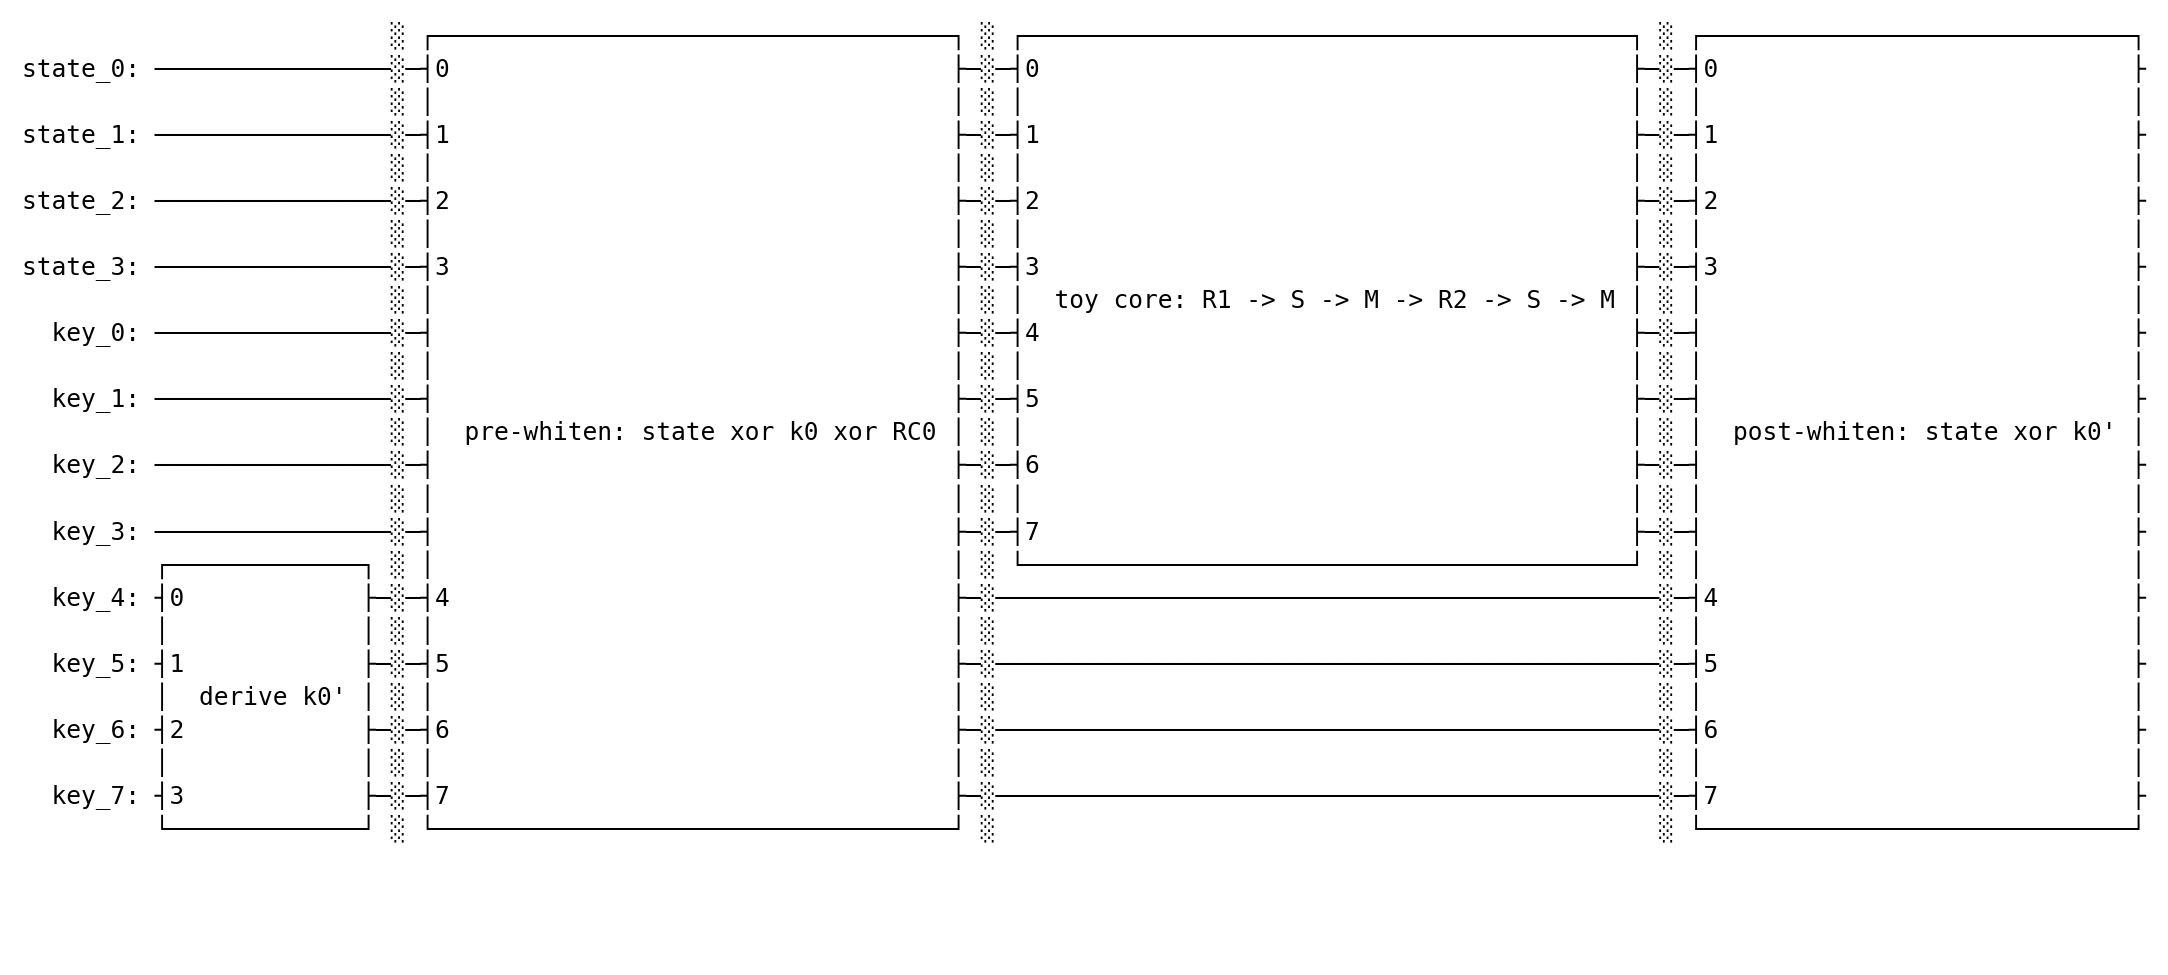
\includegraphics[width=\textwidth]{Figures/toy_prince_full_circuit.png}
\caption{Block-level circuit representation of Toy PRINCE encryption}
\label{fig:toy_prince_full_circuit}
\end{figure}

The Toy PRINCE implementation was first verified classically. The zero test confirms that the encryption and decryption routines are mutually consistent. A non-zero test uses plaintext $0x9$ and key $0x6D$, for which the key schedule gives $k_0=0x6$, $k_1=0xD$, and $k_0'=0x3$. The resulting ciphertext is $0x2$. In addition, every one of the 256 possible keys was checked over all 16 plaintext values to confirm that encryption is a permutation and that decryption recovers the original plaintext.

\begin{table}[H]
\centering
\caption{Toy PRINCE Correctness Verification}
\label{tab:toy_prince_correctness}
\small
\begin{tabularx}{\textwidth}{|X|c|c|c|c|}
\hline
\textbf{Test} & \textbf{Plaintext} & \textbf{Key} & \textbf{Ciphertext} & \textbf{Result} \\
\hline
Zero encrypt/decrypt & 0x0 & 0x00 & 0xB & PASS \\
\hline
Non-zero encrypt/decrypt & 0x9 & 0x6D & 0x2 & PASS \\
\hline
Reversibility & All 16 plaintexts & All 256 keys & -- & PASS \\
\hline
Alpha reflection & All 16 states & All 16 $k_1$ values & -- & PASS \\
\hline
\end{tabularx}
\end{table}

After correctness verification, Toy PRINCE was embedded in a Grover key-search experiment. The secret key was fixed as $0x6D$. Three known plaintext--ciphertext pairs were generated from this key and used by the oracle. The use of three pairs removes false key candidates in the 8-bit search space, leaving exactly one marked key.

\begin{table}[H]
\centering
\caption{Known Plaintext--Ciphertext Pairs Used in Toy PRINCE Grover Search}
\label{tab:toy_prince_known_pairs}
\begin{tabular}{|c|c|c|}
\hline
\textbf{Pair} & \textbf{Plaintext} & \textbf{Ciphertext under key 0x6D} \\
\hline
1 & 0x9 & 0x2 \\
\hline
2 & 0x2 & 0x4 \\
\hline
3 & 0xE & 0x3 \\
\hline
\end{tabular}
\end{table}

The Grover simulation starts with a uniform superposition over all 256 keys, so each key initially has probability $1/256 = 0.003906$. The oracle flips the phase of key $0x6D$, and the diffuser then amplifies its amplitude. The simulation was stopped when the highest key probability crossed the selected threshold of $0.99$. The correct key reached probability $0.999947$ after 12 Grover iterations.

\begin{table}
\centering
\caption{Toy PRINCE Grover Probability Amplification}
\label{tab:toy_prince_grover_summary}
\small
\begin{tabularx}{\textwidth}{|c|c|X|X|}
\hline
\textbf{Iteration} & \textbf{Most Probable Key} & \textbf{Top Key Probability} & \textbf{Marked-Key Probability} \\
\hline
0 & 0x00 & 0.003906 & 0.003906 \\
\hline
1 & 0x6D & 0.034791 & 0.034791 \\
\hline
4 & 0x6D & 0.284743 & 0.284743 \\
\hline
8 & 0x6D & 0.763722 & 0.763722 \\
\hline
10 & 0x6D & 0.935176 & 0.935176 \\
\hline
11 & 0x6D & 0.982583 & 0.982583 \\
\hline
12 & 0x6D & 0.999947 & 0.999947 \\
\hline
\end{tabularx}
\end{table}

\begin{figure}
\centering

\includegraphics[width=\textwidth]{Figures/toy_prince_grover_attack_full_circuit.png}
\caption{Block-level circuit for one Toy PRINCE Grover attack iteration}
\label{fig:toy_prince_grover_full_circuit}
\end{figure}

The Toy PRINCE experiment confirms the complete workflow used for the main PRINCE study. First, a PRINCE-like reversible cipher is defined using key whitening, S-box substitution, an M-layer, round constants, and a derived whitening key. Second, the cipher is verified for reversibility and alpha reflection. Third, the encryption circuit is used inside an oracle that marks keys consistent with known plaintext--ciphertext pairs. Finally, Grover diffusion amplifies the marked key until it dominates the measurement distribution. This small-scale experiment demonstrates the full attack mechanism that is infeasible to simulate directly for the 128-bit PRINCE key space.

\begin{figure}[h]
    \centering
    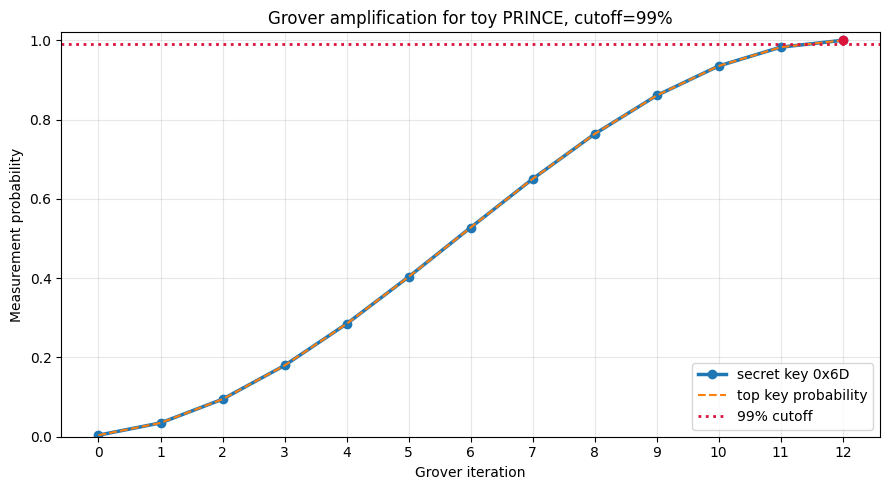
\includegraphics[width=0.65\linewidth]{Figures/Grover-amplification.png}
    \caption{Grover amplification}
    \label{fig:GroverAmplification}
\end{figure}

\section{Conclusion and Future Work}

This thesis presented a reversible quantum implementation of the PRINCE lightweight block cipher and analyzed its use within a Grover-based key search framework. A complete reversible circuit for the PRINCE encryption structure was constructed by implementing the S-box layer, M-layer, round constants, key addition operations, and the PRINCE key schedule using reversible quantum operations. The resulting circuit preserves the functional behavior of the classical PRINCE cipher while satisfying the reversibility requirements of quantum computation.

The project also showed how reversible PRINCE circuit can be implemented within the oracle circuit of the Grover algorithm to enable the quantum exhaustive search for cryptographic keys. A single Grover iteration was implemented with oracle computation, phase inversion, uncomputation, and Grover diffuser. However, as a full simulation over the whole 128-bit space of the keys would involve $2^{128}$ states, a full-state simulation was not possible on classical computer. Hence, the project concentrated on designing a circuit and evaluating its correctness and resources.

Correctness was proven by testing the equivalence between the output of the classic and quantum PRINCE implementations, as well as by demonstrating the alpha-reflection properties of PRINCE. The next step in the research was a resource analysis for the quantum PRINCE encryption circuit and a single Grover iteration. Such metrics as number of qubits, total gate count, number of layers in the circuit, number of Clifford gates, T gates, and T-depth were calculated. As it turns out, although Grover's algorithm enables an attacker to reduce the security level of a 128-bit key to 64 bits from a theoretical standpoint, its realization involves a huge number of gates, circuit depth, and fault-tolerant resources.

This work emphasizes that while there have been many theoretical studies on the ability of quantum search algorithms to break symmetric block ciphers, they do not take into account the complexities of such an operation on a practical scale. This study further proves that the post-quantum strength of symmetric block ciphers can be analyzed by designing a reversible circuit and estimating quantum resources.

There are several avenues that could be taken up as future work due to this work. The first area of focus is reducing the amount of qubits used, the number of Toffolis, the number of T-gates, and the depth of the quantum circuit designed for PRINCE. Improved S-boxes and faster implementation of linear layers in place can contribute greatly to reducing the amount of resources used.

Further research can apply this methodological approach to evaluate quantum resource consumption for lightweight block ciphers like PRESENT, GIFT, or Midori in terms of Grover’s attack. Moreover, considering realistic noise, applying quantum error correction and taking into account hardware limitations would allow us to assess whether or not quantum cryptanalysis is feasible.


\bibliographystyle{unsrt}
\bibliography{bib}
\end{document}
